\documentclass[12pt]{report}
\usepackage[T1]{fontenc}
\usepackage[french]{babel}
\usepackage[utf8x]{inputenc}
\usepackage{amsmath}
\usepackage{graphicx}
\usepackage[colorinlistoftodos]{todonotes}

\begin{document}



%-----------------------------------------------------------------%
%    PAGE DE TITRE
%-----------------------------------------------------------------%

\begin{titlepage}

\newcommand{\HRule}{\rule{\linewidth}{0.7mm}} % Trait horizontal

\center
 
%---------------------------%
%   LOGO & EN-TÊTE DE PAGE
%---------------------------%

\includegraphics[width=0.8\textwidth]{img/logo.jpg}\\

\textsc{\Large Projet de Programmation}\\[0.5cm]
\textsc{\large Génération procédurale de planètes}\\[0.5cm]

%---------------------------%
%   TITRE
%---------------------------%

\HRule \\[0.4cm]
{ \huge \bfseries Cahier des besoins}\\[0.4cm]
\HRule \\[1.5cm]
 
%---------------------------%
%   AUTHEURS
%---------------------------%

\begin{minipage}{0.4\textwidth}
\begin{flushleft} \large
\emph{Auteurs:}\\
Rémy \textsc{Maugey}\\
Jérémi \textsc{Bernard}\\
Hugo \textsc{Alonso}\\
Brian \textsc{Mazé}\\
\end{flushleft}
\end{minipage}
~
\begin{minipage}{0.4\textwidth}
\begin{flushright} \large
\emph{Client:} \\
Emmanuel \textsc{Fleury}
\end{flushright}
~
\begin{flushright} \large
\emph{Chargé de TD:} \\
Boris \textsc{Mansencal}
\end{flushright}
\end{minipage}\\[2cm]

%---------------------------%
%   DATE
%---------------------------%

{\large 22 Janvier 2018}\\[2cm] 


\vfill % Fill the rest of the page with whitespace

\end{titlepage}
%-----------------------------------------------------------------%
%   FIN PAGE DE TITRE
%-----------------------------------------------------------------%

%-----------------------------------------------------------------%
%   Table des Matières
%-----------------------------------------------------------------%


\tableofcontents

\thispagestyle{empty} % empeche l'affichage du numero de cet page

%-----------------------------------------------------------------%
%   Introduction
%-----------------------------------------------------------------%

\newpage

\chapter*{Introduction}
\addcontentsline{toc}{chapter}{Introduction}
\setcounter{chapter}{1}

Un objet en trois dimensions complexe est un ensemble de sommets reliés
entre eux par des arrêtes, formant des faces triangulaires. L'ensemble
de ces points et arrêtes est appelé maillage. Ces triangles sont ensuite
traités et affichés à l'écran en deux dimensions. Plus le nombre de
triangles à afficher est élevé, plus le rendu d'une image est long, ce
qui est problématique dans une application nécessitant de générer
beaucoup d'images rapidement, par exemple pour un rendu temps réel dans
une simulation ou un jeu vidéo.\\
Il est alors intéressant de pouvoir réduire le nombre de triangles d'un
objet qui n'a pas besoin d'être très détaillé dans un cas précis, par
exemple si l'objet est loin de l'observateur. Un cas particulier est
l'affichage d'une surface très grande comportant des aspérités, par
exemple un terrain. Une partie du terrain est proche de l'observateur,
nous voulons donc en afficher les détails, mais une autre partie est
plus éloignée, et les détails seront moins visibles sur l'image finale.
On peut donc réduire le nombre de triangle de la partie éloignée afin de
réduire le nombre de triangles à traiter.

L'objectif de ce projet est d'implémenter un système de \emph{LOD} (
\emph{Level of Detail}: niveau de détail) à appliquer sur le maillage
d'une sphère en vue d'une application en temps réel, afin d'optimiser
son affichage. Ce système sera fournis en temps que bibliothèque de
fonctions.
Le projet comportera aussi une application permettant le rendu de cette
sphère en trois dimensions, afin de pouvoir visualiser le fonctionnement
du système de \emph{LOD}, ainsi qu'un moyen de mesurer les performances
du système. Comme demandé, notre projet se basera sur la méthode
proposée dans \cite{CDLOD}, permettant de générer le maillage en temps
réel en fonction de la distance à la caméra. 

%-----------------------------------------------------------------%
%   État de l’existant
%-----------------------------------------------------------------%
\newpage

\chapter*{État de l'existant}
\addcontentsline{toc}{chapter}{État de l'art}
\setcounter{chapter}{2}

%L'objectif final du projet est d'optimiser l'affichage de la planète
%grâce à un système de niveau de détails variant en fonction de
%l'éloignement de la caméra. Plusieurs implémentations allant dans ce
%sens existent et ont déja été publiées.  Notre projet sera basé sur la
%technique décrite par Filip Strugar en 2010, \textit{Continuous
%Distance Dependent Level of Detail for Rendering Heightmaps}.  D'autre
%projets similaires existent mais utilisent des structures de données
%différentes, l'utilisation d'un système de \textbf{chunks} ou encore de
%\textbf{clipmaps}. Bien que toutes ces techniques soient différentes,
%elles se basent sur le même principe fondamental, rajouter à la volée
%des détails sur les objets proches.

%Nous adapterons la méthode de \cite{CDLOD} qui utilise le \emph{GPU}
%pour développer une version \emph{CPU}. Cette méthode a l'avantage de
%rattacher les maillages des différents niveau de détail de manière lisse
%et progressive, c'est à dire sans frontières intermédiaires, rendant le
%résultat homogène. Un autre avantage de cette méthode est de garder le
%nombre de triangles affichés constant, en répartissant les triangles
%dans les différents niveaux de détails.

De nombreuses applications utilisent des techniques d'optimisation de
l'affichage. Notamment les applications qui demandent de bonnes
performances tel que les simulations 3D ou les jeux vidéos.
%Génération Procédural
Dans le cas du développement d'un environnement 3D il est souvent fait
appel à des techniques de génération procédural, par exemple le logiciel
Terragen qui est utilisé dans le monde du cinéma ou encore Elite
dangerous dans le monde du jeux vidéos.  Ces deux applications utilisent
des mécanisme de génération procédurale pour créer respectivement des
planètes et une galaxie.
%% TODO: Mettre en référence Terragen et Elite Dangerous dans la Bib

%LOD et dérivé
Plusieurs algorithmes peuvent être utilisé dans la mise en place d'un
système de niveau de détail dynamique, tous d'abord le \cite{CDLOD} qui
est utilisé comme référence dans le cadre de se projet. Ce dernier sera
adapté car il utilise le \emph{GPU}. Il a l'avantage de rattacher les
maillages des différents niveaux de détails de manière lisse et
progressive c'est à dire sans frontières intermédiaires, rendant le
résultat homogène.  Un autre avantage de cette méthode est de garder le
nombre de triangles affichés constant, en répartissant les triangles
dans les différents niveaux de détails.\\
Une autre approche serait de mettre à jour des zones entière de terrain,
comme détaillé par \cite{MassiveTerrain}. Cet algorithme ne permet pas
de garder un nombre constant de triangles affichés par le fait qu'ils
s'affichent par groupe. Il est aussi implémenté sur \emph{GPU}.\\


%http://tulrich.com/geekstuff/sig-notes.pdf
%http://hhoppe.com/gpugcm.pdf
%http://dept-info.labri.fr/~narbel/PdP/Subjects17-18/Papers/cdlod_latest.pdf

%-----------------------------------------------------------------%
%   ANALYSE DES BESOINS
%-----------------------------------------------------------------%
\newpage

\chapter*{Analyse des besoins}
\addcontentsline{toc}{chapter}{Analyse des besoins}
\setcounter{chapter}{3}

%% Trier les besoins :

% Créer une structure de données quadtree
% Stocker des heightmaps dans les quadtree
% Générer des heightmaps
% Crééer une lib pour gérer les quadtrees (voir ça comme une base de données) => demande(theta, rho) => DB => return z;
% Convertir les coordonnées x,y de la heightmap en coordonnées polaires
	% x = rho cos theta
    % y = rho sin theta

% Récupérer la hauteur z dans le quadtree
% Faire une sphère avec un maillage hiérarchique
% Afficher la sphère avec opengl
% Paramètre de l'application : -d Density -i Init point
% Faire les tests unitaires // pourquoi (hugo)? L'appli a pas besoin d’être robuste. Les test unitaires seront durs à implémentés
% Test de performance (en fonction de la densité)
% Afficher un compteur de fps
% Densité changeable en live (par ex avec + et -), peut être afficher aussi la densité
% Doc et commentaire en anglais
% CI avec travis, style de codage cohérent
% Utilisation de triangle pour représenter le maillage

% Se déplacer dans la scène 3d
%Gérer les événements clavier et souris. Les mettre en relation avec une classe caméra. Prendre en compte cette caméra dans la boucle d'affichage de la sphère afin de pouvoir se déplacer dans la scène 3D.

%---------------------------%
%   BESOINS FONCTIONNELS
%---------------------------%

\section{Besoins fonctionnels}

\subsection{Génération de terrain}

Générer aléatoirement la carte de hauteur d'un terrain. 
Nous aurons besoin d'une méthode pour traduire les points dans la heightmap en point cartésiens 3D.
Pour cela, nous comptons pour l'instant prendre le premier point de la heightmap et le mappé sur une une vrai coordonnée 3d (non nul). Pour retrouver la position 3D du point P (x,y), il suffit d'éxécuter une rotation proportionnelle en x et en y du vecteur formé par le mappé le centre de la planete. Ensuite, on norme le vecteur à la valeur contenue dans la height map. 


\subsection{Interface graphique}

Afficher à l'écran une scène en trois dimensions représentant la planète.\\
La surface de la planète sera affichée en maillage, afin de bien voir
les triangles créés par l'algorithme.\\
Déplacer la caméra dans l'espace en fonction des entrées clavier et
souris de l'utilisateur.\\
Afficher dans un coin de l'écran les informations sur les performances
sous forme du nombre d'images par seconde.\\

\subsection{Structure de donnée}

Implémenter une structure de donnée représentant un quadtree pour
l'algorithme de CDLOD (voir figure \ref{fig:quadtree} tirée de 
\cite{CDLOD}).\\
Un quadtree est un arbre dont chaque nœud possède quatre fils, cette
structure de donnée nous permet de subdiviser le terrain, chaque nœud
représentant une surface du terrain. Une nœud contient la représentation
de sa zone à son niveau de détail, et quatre fils représentant chacun un
quart de la zone du parent au niveau de détail supérieur.\\

\begin{figure}[!h]
  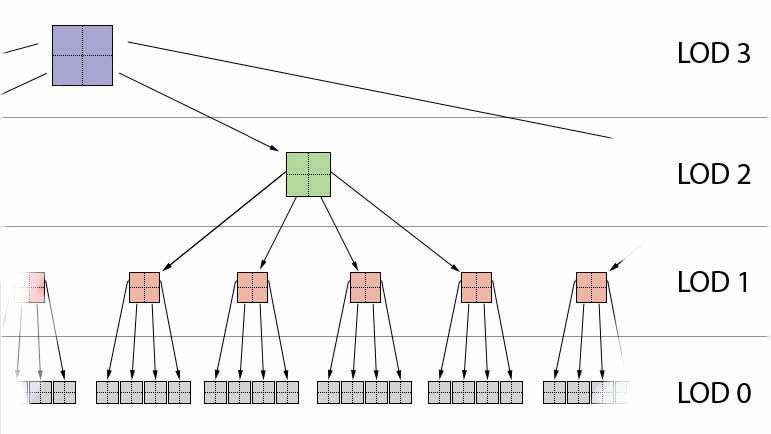
\includegraphics[scale=0.5]{img/Quadtree.png}
  \caption{Quadtree \cite{CDLOD}}
  \label{fig:quadtree}
\end{figure}

\subsection{CDLOD}

Implémenter un algorithme inspiré de \cite{CDLOD}, conformément aux
demandes du client.\\
L'algorithme permettra de générer les différents niveaux de détails de
la surface de la planète, et sera accessible dans une bibliothèque
séparée du reste du projet.\\
La structure de donnée et les algorithmes correspondant seront fournis
indépendamment de la partie affichage graphique dans une interface de
programmation.\\
L'API peut être vue comme une base de donnée, des requêtes sont faites
en lui donnant comme données de départ deux coordonnées polaire
représentant une zone sur la sphère ainsi que les coordonnées de la
caméra.\\
La bibliothèque retournera un arbre composé des différentes cartes de
hauteurs.\\

\subsection{Mesure des performances}

Mesurer le nombre d'images générées par seconde, les afficher à l'écran.\\
Mesurer le temps de réponse de la bibliothèque à chaque requête.\\
Afficher les résultats dans la sortie standard à la fin de l'exécution
du programme.\\

%---------------------------%
%   BESOINS NON FONCTIONNELS
%---------------------------%

\section{Besoins non fonctionnels}

\subsection{Intégration continue}

Mettre en place un système d'intégration continue en parallèle au projet
afin d'exécuter les tests.\\

\subsection{Gestionnaire de versions}

Utiliser un outil de gestion de version afin de disposer d'un dépôt
partagé et de suivre l'évolution du projet.\\

\subsection{Documentations}

Documenter les interfaces du projets ainsi que les implémentations, en
anglais.\\

\subsection{Tests}

Mettre en place des tests unitaires.\\
Tout les tests seront utilisés au long du projet afin de vérifier que
les nouvelles fonctionnalités apportées ne dérangent pas le bon
fonctionnement des précédentes.

%-----------------------------------------------------------------%
%   MISE EN OEUVRE
%-----------------------------------------------------------------%
\newpage

\chapter*{Mise en Oeuvre}
\addcontentsline{toc}{chapter}{Mise en Oeuvre}
\setcounter{chapter}{4}



%---------------------------%
%   DIAGRAMME DE GRANT
%---------------------------%

\section{Diagramme de Gantt}

\begin{figure}[!h]
  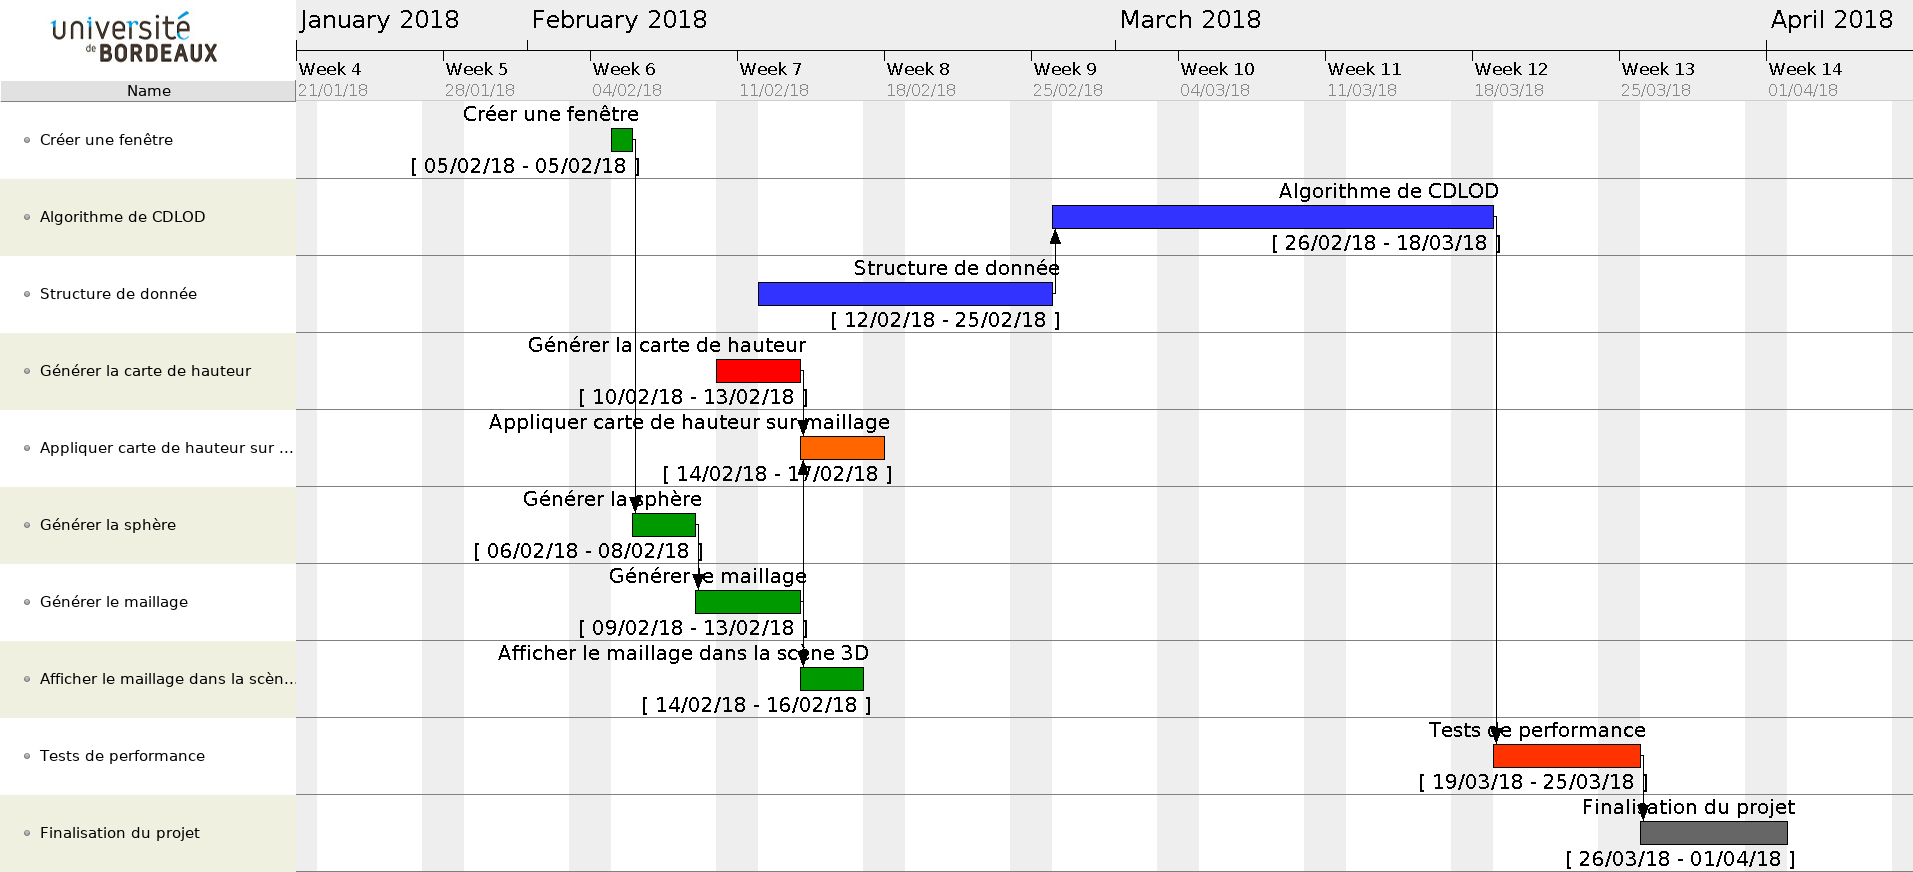
\includegraphics[scale=0.5]{img/gantt.png}
  \caption{Diagramme de Gantt}
  \label{fig:gantt}
\end{figure}

\bibliography{biblio}{}
\bibliographystyle{plainnat}


\end{document}
